%\chapter{Procedure call and data mapping for procedure argument}
\chapter{Procedure Interfaces}
\label{chap:procedure}
\index{procedure interface}

This chapter describes the procedure interfaces, that is, how
procedures are invoked and arguments are passed, in {\XMP}.

In order to achieve high composability of {\XMP} programs, it is one of
the most important requirement that {\XMP} procedures can invoke
procedures written in the base language with as a few restrictions as
possible.
%The procedure interfaces in {\XMP} is designed so as to
%satisfy the requirement.


\section{General Rule}

In {\XMP}, a procedure invocation itself is a local operation and does
not cause any communication or synchronization at runtime. Thus, a node
can invoke any procedure, whether written in {\XMP} or in the base
language, at any point of the execution.
%
There is no restriction on the characteristics of procedures invoked by
an {\XMP} procedure, except for a few ones on its argument, which is
explained below.

A local data in the actual or dummy argument list (referred to as a {\it
\Term{local actual argument}} and a {\it \Term{local dummy argument}},
respectively) are treated by the {\XMP} compiler in the same manner as
by the compiler of the base language.
%
This rule makes it possible that a local actual argument in a procedure
written in {\XMP} can be associated with a dummy argument of a procedure
written in the base language.

If both of an actual and its associating dummy arguments are coarrays,
they must be declared on the same node set.


\paragraph*{Implementation.}

The {\XMP} compiler does not transform either local actual or dummy
arguments, so that the backend compiler of the base language can treat
them in its usual way.

\vspace{1.5zw}

\hspace{-1.2\parindent}
The rest of this chapter specifies how global data appearing as an
actual and a dummy argument list (referred to as a {\it \Term{global actual
argument}} and a {\it \Term{global dummy argument}}, respectively) are
processed by the {\XMP} compiler.


\section{Argument Passing Mechanism in {\XMP} Fortran}

%Any section (except for an element) of a global data may not be put in
%the actual argument list. Therefore only the name or an element of it
%may be put in the actual argument list.

Either of the following global data can be put in the actual argument list:

\begin{itemize}
 \item an array name;
 \item an array element; or
 \item an array section that satisfies both of the following two
       conditions:
       \begin{itemize}
	\item its subscript list is a list of zero or more colons
	      (``{\tt :}'') followed by zero or more {\it int-expr}'s;
	\item a subscript of the dimension having shadow is {\it
	      int-expr} unless it is the last dimension.
       \end{itemize}
\end{itemize}

There are two kinds of argument association for global data in {\XMP}
Fortran: one is {\it \Term{sequence association}}, which is for a global
dummy that is an explicit-shape or assumed-size array, and the other is
{\it \Term{descriptor association}}, which is for all other global dummy.


\subsection{Sequence Association of Global Data}
\index{sequence association}

The concept of sequence association in {\Fort} is extended for global
actual and dummy arguments in {\XMP} as follows.

If the actual argument is an array name or an array section that
satisfies the above conditions, it represents an element sequence
consisting of the elements of its local section in Fortran's array
element order on each node.
%
Also, if the actual argument is an element of a global data, it
represents an element sequence consisting of the corresponding element
in the local section and each element that follows it in array element
order on each node.

An global actual argument that represents an element sequence and
corresponds to a global dummy argument is sequence associated with
the the dummy argument if the dummy argument is an explicit-shape or
assumed-size array.
%
According to this (extended) sequence association rule, each element of
the element sequence represented by the global actual argument is
associated with the element of the local section of the global dummy
argument that has the same position in array element order.

Sequence association is the default rule of association for global
actual arguments and therefore is applied unless it is obvious from the
interface of the invoked procedure that the corresponding dummy argument
is neither an explicit-shape nor assumed-size array.


\paragraph*{Implementation.}

In order to implement sequence association, the name, a section, or an
element of a global data appearing as an actual argument is treated by
the {\XMP} compiler as the base address of its local section on each
node, and the global data appearing as the corresponding dummy argument
is initialized at runtime so as to be composed of the local sections
each of which starts from the address received as the argument.
%
On a node that does not have the local section corresponding to the
actual argument, an unspecified value (e.g. null) is received.

Such implementation implies that in many cases, in order to associate
properly a global actual argument with the global dummy argument, their
mappings (including their shadow attributes) must be identical.


\subsubsection*{Examples}
\index{Example!procedure interface}

\begin{description}

\item[Example 1]

	   Both the actual argument {\tt a} and the dummy argument {\tt
	   x} are global explicit-shape arrays, and therefore {\tt
	   a} is sequence associated with {\tt x}.

	   It is the base address of the local section of {\tt a} that
	   passed between these subroutines on each node. Each the local
	   section of {\tt x} starts from the received address (Figure
	   \ref{fig5.1}).

\begin{XFexample}
      subroutine xmp_sub1
!$xmp nodes p(4)
!$xmp template t(100)
!$xmp distribute t(block) onto p
      real a(100)
!$xmp align a(i) with t(i)
!$xmp shadow a(1:1) 
      call xmp_sub2(a)
      end subroutine

      subroutine xmp_sub2(x)
!$xmp nodes p(4)
!$xmp template t(100)
!$xmp distribute t(block) onto p
      real x(100)
!$xmp align x(i) with t(i)
!$xmp shadow x(1:1) 
      ...
\end{XFexample}

\begin{myfigure}
 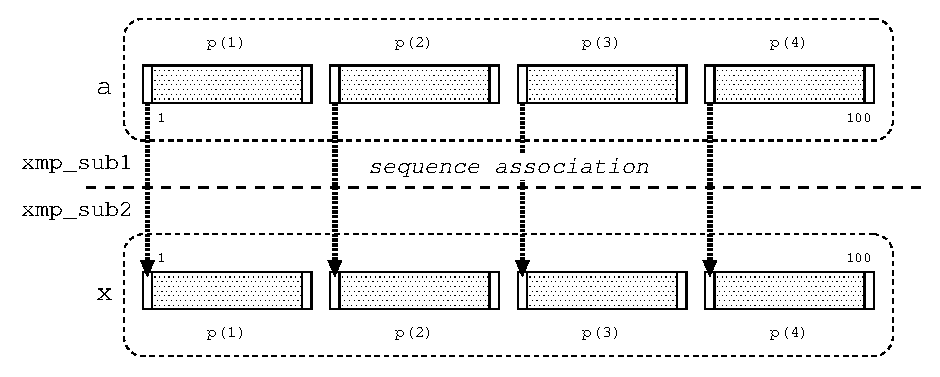
\includegraphics[scale=0.7]{figs/fig5.1.eps}
 \caption{Sequence Association with a Global Dummy Argument}
 \label{fig5.1}
\end{myfigure}

\item[Example 2]

	   The actual argument {\tt a} is a global explicit-shape array,
	   and the dummy argument {\tt x} is a local explicit-shape. 
	   Sequence association is applied also in this case.

	   The caller subroutine {\tt xmp\_sub1} passes the base address
	   of the local section of {\tt a} on each node, and the callee
	   {\tt f\_sub2} receives it and initializes {\tt x} with the
	   storage starting from it (Figure \ref{fig5.2}).

\begin{XFexample}
      subroutine xmp_sub1
!$xmp nodes p(4)
!$xmp template t(100)
!$xmp distribute t(block) onto p
      real a(100)
!$xmp align a(i) with t(i)
!$xmp shadow a(1:1) 
      n = 1 + 100/4 + 1
      call f_sub2(a,n)
      end subroutine
\end{XFexample}
\begin{Fexample}
      subroutine f_sub2(x,n)
      real x(n)
      ...
\end{Fexample}

\begin{myfigure}
 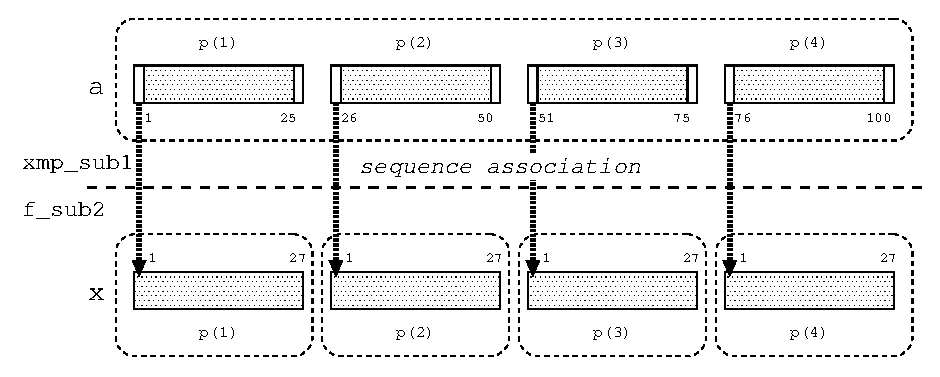
\includegraphics[scale=0.7]{figs/fig5.2.eps}
 \caption{Sequence Association with a Local Dummy Argument}
 \label{fig5.2}
\end{myfigure}

\item[Example 3]

	   The actual argument {\tt a(:,1)} is a contiguous section of
	   the global data, and the dummy argument {\tt x} is a local
	   explicit-shape array. Sequence association is applied 
	   in this case, but only the node {\tt p(1)} owns the section.
	   Hence, {\tt f\_sub2} is invoked only by {\tt p(1)} (Figure
	   \ref{fig5.25}).

\begin{XFexample}
      subroutine xmp_sub1
!$xmp nodes p(4)
!$xmp template t(100,100)
!$xmp distribute t(*,block) onto p
      real a(100,100)
!$xmp align a(i,j) with t(i,j)
!$xmp shadow a(0,1:1)
      n = 100
!$xmp task on p(1)
      call f_sub2(a(:,1),n)
!$xmp end task
      end subroutine
\end{XFexample}
%
\begin{Fexample}
      subroutine f_sub2(x,n)
      real x(n)
      ...
\end{Fexample}

\clearpage

\begin{myfigure}
 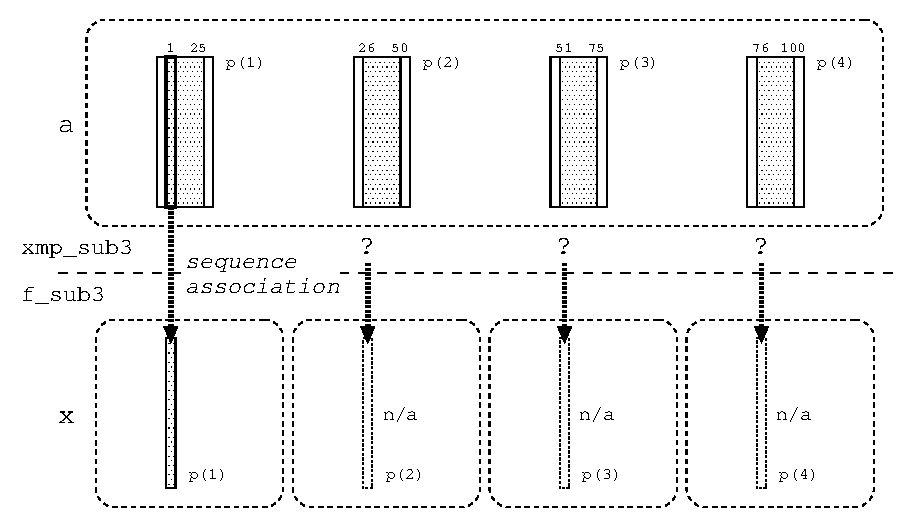
\includegraphics[scale=0.7]{figs/fig5.25.eps}
 \caption{Sequence Association of a Section of a Global Data as an
 Actual Argument with a Local Dummy Argument}
 \label{fig5.25}
\end{myfigure}

\item[Example 4]

	   The actual argument {\tt a(1)} is an element of the global
	   data, and the dummy argument {\tt x} is a local
	   explicit-shape array. Sequence association is applied 
	   in this case, but only the node {\tt p(1)} owns the element.
	   Hence, {\tt f\_sub2} is invoked only by {\tt p(1)}(Figure
	   \ref{fig5.3}).

\begin{XFexample}
      subroutine xmp_sub1
!$xmp nodes p(4)
!$xmp template t(100)
!$xmp distribute t(block) onto p
      real a(100)
!$xmp align a(i) with t(i)
!$xmp shadow a(1:1)
      n = 100/4
!$xmp task on p(1)
      call f_sub2(a(1),n)
!$xmp end task
      end subroutine
\end{XFexample}
%
\begin{Fexample}
      subroutine f_sub2(x,n)
      real x(n)
      ...
\end{Fexample}

\begin{myfigure}
 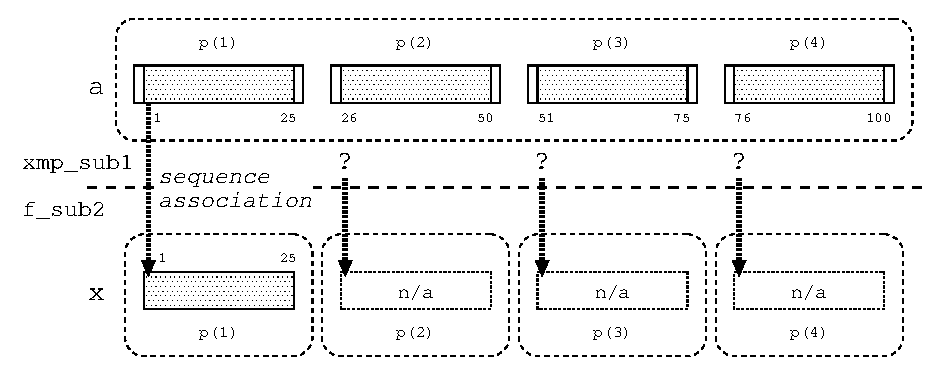
\includegraphics[scale=0.7]{figs/fig5.3.eps}
 \caption{Sequence Association of an Element of a Global Data as an
 Actual Argument with a Local Dummy Argument}
 \label{fig5.3}
\end{myfigure}

\item[Example 5]

	   Even if either the global actual or dummy argument has a full
	   shadow, the sequence association rule is the same in
	   principle. Hence, the base address of the local section of
	   {\tt a} is passed between these subroutines on each node, and
	   each the local section of {\tt x} starts from the received
	   address (Figure \ref{fig5.4}).

\begin{myfigure}
 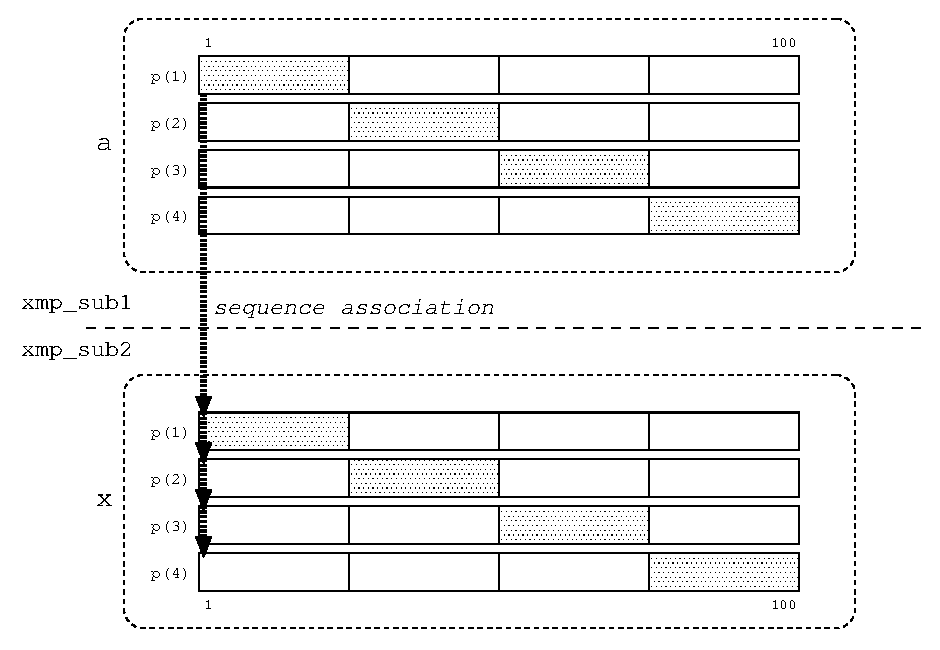
\includegraphics[scale=0.7]{figs/fig5.4.eps}
 \caption{Sequence Association with a Global Dummy Argument that Has
 Full Shadow}
 \label{fig5.4}
\end{myfigure}

\end{description}


\subsection{Descriptor Association of Global Data}
\index{descriptor association}

When the actual argument is a global data and it is obvious from the
interface of the invoked procedure that the corresponding dummy argument
is neither an explicit-shape nor assumed-size array, the actual
argument is {\it descriptor associated} with the dummy
argument. According to the descriptor association rule, the dummy
argument inherits its shape and storage from the actual argument.

\paragraph*{Implementation.}

In order to implement the descriptor association, a global actual
argument is treated by the {\XMP} compiler:

\begin{itemize}
 \item as if it were the {\it global-data descriptor} of the actual array, 
       which is an internal data structure managed by the {\XMP} runtime
       system to hold information on a global data (see \ref{subsec:
       xmp_desc_of}), if the dummy is a global data; or
 \item as it is an array representing the local section of the actual
       array, which is to be processed by the backend Fortran compiler
       in the same manner as usual data, if the dummy is a local data.
\end{itemize}

For the first case, a global dummy is initialized at runtime with a copy
of the global-data descriptor received.

When an actual argument is descriptor associated with the dummy argument
and their mappings are not identical, the {\XMP} runtime system may
detect and report the error.

\subsubsection*{Examples}
\index{Example!procedure interface}

\begin{description}

\item[Example 1]

	   There is the explicit interface of the subroutine
	   {\tt xmp\_sub2} specified by an interface block in the
	   subroutine {\tt xmp\_sub1}, from which it is found that the
	   dummy argument {\tt x} is a global assumed-shape
	   array. Therefore the global actual argument {\tt a} is
	   descriptor associated with the global dummy argument {\tt
	   x}.

	   It is the global-data descriptor of {\tt a} that passed
	   between these subroutines. The dummy argument {\tt x} is
	   initialized by the {\XMP} runtime system on the basis of the
	   information extracted from the descriptor received (Figure
	   \ref{fig5.5}).

\begin{XFexample}
      subroutine xmp_sub1

!$xmp nodes p(4)
!$xmp template t(100)
!$xmp distribute t(block) onto p
      real a(100)
!$xmp align a(i) with t(i)
!$xmp shadow a(1:1)

      interface
      subroutine xmp_sub2(x)
!$xmp nodes p(4)
!$xmp template t(100)
!$xmp distribute t(block) onto p
      real x(:)
!$xmp align x(i) with t(i)
!$xmp shadow a(1:1)
      end subroutine xmp_sub2
      end interface

      call xmp_sub2(a)

      end subroutine

      subroutine xmp_sub2(x)
!$xmp nodes p(4)
!$xmp template t(100)
!$xmp distribute t(block) onto p
      real x(:)
!$xmp align x(i) with t(i)
!$xmp shadow a(1:1)
      ...
\end{XFexample}

\begin{myfigure}
 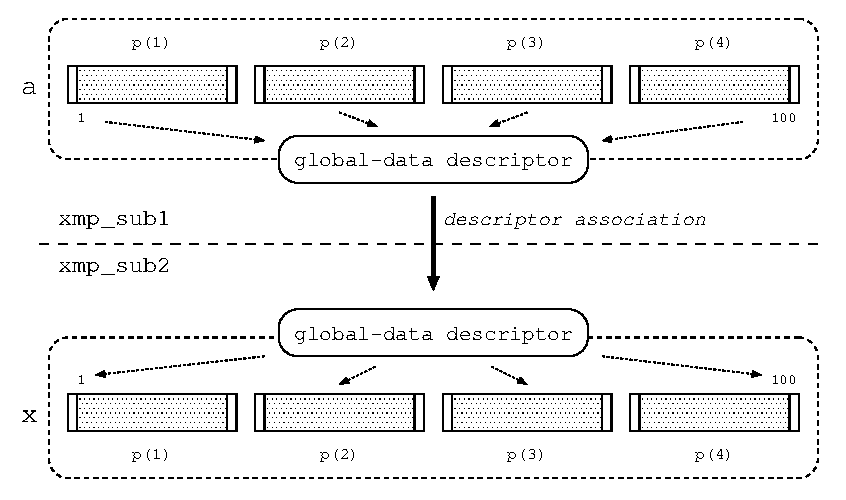
\includegraphics[scale=0.7]{figs/fig5.5.eps}
 \caption{Descriptor Association with a Global Dummy Argument}
 \label{fig5.5}
\end{myfigure}

\item[Example 2]

	   There is the explicit interface of the subroutine
	   {\tt f\_sub2}, which is written in {\Fort},
	   specified by an interface block in the subroutine {\tt
	   xmp\_sub1}, and the dummy argument {\tt x} is a local
	   (i.e. non-mapped) assumed-shape array. Therefore the global
	   actual argument {\tt a} is descriptor associated with the
	   local dummy argument {\tt x}.

	   The global actual argument is replaced with its local section
	   by the {\XMP} compiler and the association of the local
	   section with the dummy argument is to be processed by the
	   backend Fortran compiler in the same manner as usual data 
	   (Figure \ref{fig5.6}).

\begin{XFexample}
      subroutine xmp_sub1

!$xmp nodes p(4)
!$xmp template t(100)
!$xmp distribute t(block) onto p
      real a(100)
!$xmp align a(i) with t(i)
!$xmp shadow a(1:1) 

      interface
      subroutine f_sub2(x)
      real x(:)
      end subroutine f_sub2
      end interface

      call f_sub2(a)

      end subroutine
\end{XFexample}
\begin{Fexample}
      subroutine f_sub2(x)
      real x(:)
      ...
\end{Fexample}

\begin{myfigure}
 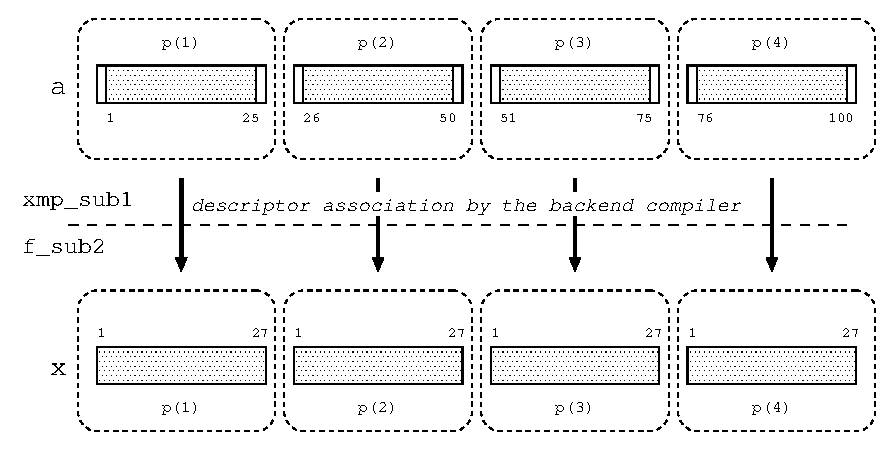
\includegraphics[scale=0.7]{figs/fig5.6.eps}
 \caption{Descriptor Association with a Local Dummy Argument}
 \label{fig5.6}
\end{myfigure}

\end{description}


\section{Argument Passing Mechanism in {\XMP} C}

When an actual argument is a global data, it is passed by the address
of its local section.
%
When a dummy argument is a global data, an address is received and
used as the base address of each of its local section.


\paragraph*{Implementation.}

The name of a global data appearing as an actual argument is
treated by the {\XMP} compiler as the pointer to the first element of
its local section on each node.
%
On a node onto which no part of the global data is mapped, the pointer
is set to an unspecified value (e.g. null).
%
Note that an element of a global data in the actual argument list is
treated in the same manner as those in other usual statements because an
array element is passed by value as in C.

The name of a global data appearing as a dummy argument is
treated by the {\XMP} compiler as the pointer to the first element of
its local section on each node.
%
As a result, it is initialized at runtime so as to be
composed of the local sections on the executing nodes.

Such implementation implies that in many cases, in order to pass
properly a global actual argument to the corresponding global dummy 
argument, their mappings (including their shadow attributes) must be
identical.

\subsubsection*{Examples}
%\index{Example!procedure interface}

\begin{description}

\item[Example 1]

The global actual argument {\tt a} is treated by the {\XMP}
compiler as the pointer to the first element of its local
section, which is passed to the callee, on each node.

The global dummy argument {\tt x} is initialized so that each
of its local section starts from the address held by the
received pointer (Figure \ref{fig5.7}).

\begin{XCexample}
void xmp_func1()
{
#pragma xmp nodes p[4]
#pragma xmp template t[100]
#pragma xmp distribute t[block] onto p
  float a[100];
#pragma xmp align a[i] with t[i]
#pragma xmp shadow a[1:1]

  xmp_func2(a);
}

void xmp_func2(float x[100])
{
#pragma xmp nodes p[4]
#pragma xmp template t[100]
#pragma xmp distribute t[block] onto p
#pragma xmp align x[i] with t[i]
#pragma xmp shadow a[1:1]
  ...
\end{XCexample}

\begin{myfigure}
 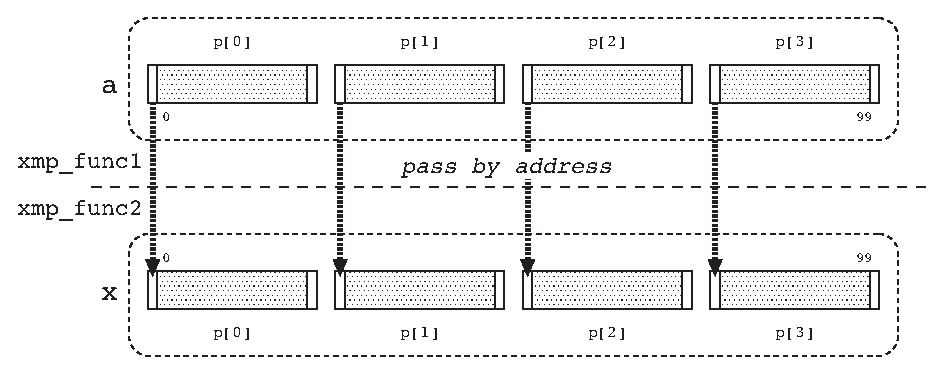
\includegraphics[scale=0.7]{figs/fig5.7.eps}
 \caption{Passing to a Global Dummy Argument}
 \label{fig5.7}
\end{myfigure}

\item[Example 2]

The global actual argument {\tt a} is treated by the {\XMP}
compiler as the pointer to the first element of its local
section, which is passed to the callee, on each node.

The local dummy argument {\tt x} on each node starts from the 
address held by the received pointer (Figure \ref{fig5.8}).

\begin{XCexample}
void xmp_func1()
{
#pragma xmp nodes p[4]
#pragma xmp template t[100]
#pragma xmp distribute t[block] onto p
  float a[100];
#pragma xmp align a[i] with t[i]
#pragma xmp shadow a[1:1]

  c_func2(a);
}
\end{XCexample}
\begin{Cexample}
void c_func2(float x[27])
{
  ...
\end{Cexample}

\begin{myfigure}
 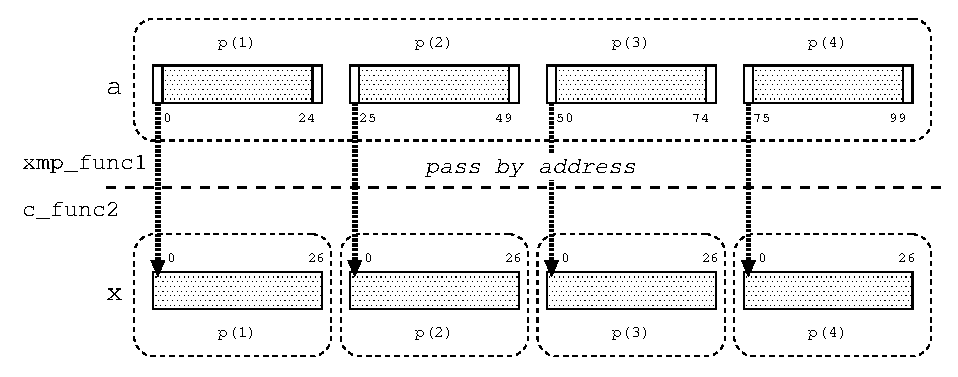
\includegraphics[scale=0.7]{figs/fig5.8.eps}
 \caption{Passing to a Local Dummy Argument}
 \label{fig5.8}
\end{myfigure}

\item[Example 3]

The actual argument {\tt a[0]} is an element of the global
data and the dummy argument {\tt x} is a scalar, in which
case the normal argument-passing rule of {\C} for variables
of a basic type (i.e. ``pass-by-value'') is applied. However,
only the node {\tt p[0]} owns the element.
Hence, {\tt c\_func2} is invoked only by {\tt p[0]} (Figure \ref{fig5.9}).

\begin{XCexample}
void xmp_func1()
{
#pragma xmp nodes p[4]
#pragma xmp template t[100]
#pragma xmp distribute t[block] onto p
  float a[100];
#pragma xmp align a[i] with t[i]
#pragma xmp shadow a[1:1]

#pragma xmp task on p[0]
  c_func2(a[0]);
}
\end{XCexample}
\begin{Cexample}
void c_func2(float x)
{
  ...
\end{Cexample}

\begin{myfigure}
 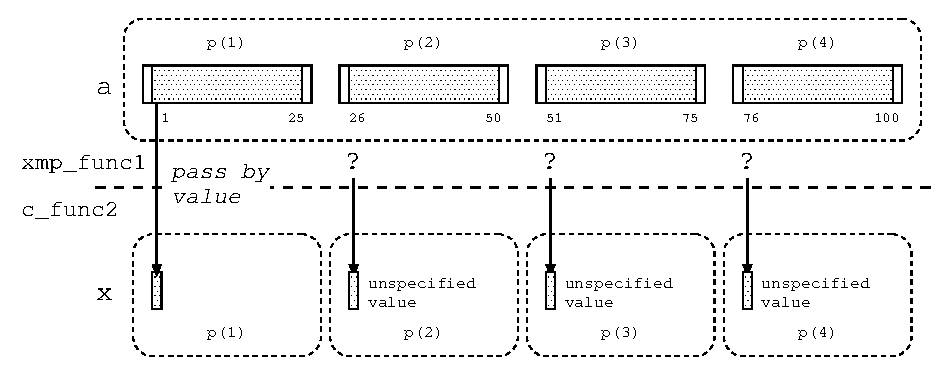
\includegraphics[scale=0.7]{figs/fig5.9.eps}
 \caption{Passing an Element of a Global Data as an Actual Argument to a
 Local Dummy Argument}
 \label{fig5.9}
\end{myfigure}

\end{description}
